\begin{ex}
(Ufrs) Sendo A um ponto fixo de um círculo de raio r e escolhendo-se ao acaso um ponto B sobre o círculo, a probabilidade da corda $\overline {AB}$  ter comprimento maio que r está entre:
   \begin{enumerate}[(a)]
   \item 25\% e 30\%
   \item 35\% e 40\%
   \item 45\% e 50\%
   \item 55\% e 60\%
   \item 65\% e 70\%
   \end{enumerate}
     \begin{sol}
      resposta: e \\ \\
      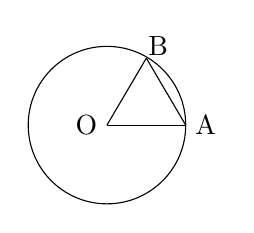
\begin{tikzpicture}
      \draw (0,0) circle [radius=1]; \draw (0,0)--(1,0);\node at (1,0) [right] {A};\node at (0,0) [left] {O}; \draw (0,0)--(.5,.85);\node at (.65,1) {B};\draw (1,0)--(.5,.85);
      \end{tikzpicture}
      $\overline{OA}=\overline{OB}=\overline{AB}=r$ \\
      O ângulo AOB mede $60^{\circ}$. Para a corda AB ser maior que \textit{r}, o ângulo AOB deve ser maior que $60^{\circ}$ e menor que $300^{\circ} \Longrightarrow p= \frac{300-60}{360}=\frac{2}{3}=66,6\%$
     
     \end{sol}
\end{ex}